\documentclass[journal,12pt,twocolumn]{IEEEtran}
%
\usepackage{setspace}
\usepackage{gensymb}
\usepackage{xcolor}
\usepackage{polynom}
\usepackage{caption}
%\usepackage{subcaption}
%\doublespacing
\singlespacing

%\usepackage{graphicx}
%\usepackage{amssymb}
%\usepackage{relsize}
\usepackage[cmex10]{amsmath}
\usepackage{mathtools}
%\usepackage{amsthm}
%\interdisplaylinepenalty=2500
%\savesymbol{iint}
%\usepackage{txfonts}
%\restoresymbol{TXF}{iint}
%\usepackage{wasysym}
\usepackage{hyperref}
\usepackage{amsthm}
\usepackage{mathrsfs}
\usepackage{txfonts}
\usepackage{stfloats}
\usepackage{cite}
\usepackage{cases}
\usepackage{subfig}
%\usepackage{xtab}
\usepackage{longtable}
\usepackage{multirow}
%\usepackage{algorithm}
%\usepackage{algpseudocode}
%\usepackage{enumerate}
\usepackage{enumitem}
\usepackage{mathtools}
%\usepackage{iithtlc}
%\usepackage[framemethod=tikz]{mdframed}
\usepackage{listings}

\let\vec\mathbf
\newcommand{\myvec}[1]{\ensuremath{\begin{pmatrix}#1\end{pmatrix}}}

%\usepackage{stmaryrd}


%\usepackage{wasysym}
%\newcounter{MYtempeqncnt}
\DeclareMathOperator*{\Res}{Res}
%\renewcommand{\baselinestretch}{2}
\renewcommand\thesection{\arabic{section}}
\renewcommand\thesubsection{\thesection.\arabic{subsection}}
\renewcommand\thesubsubsection{\thesubsection.\arabic{subsubsection}}

\renewcommand\thesectiondis{\arabic{section}}
\renewcommand\thesubsectiondis{\thesectiondis.\arabic{subsection}}
\renewcommand\thesubsubsectiondis{\thesubsectiondis.\arabic{subsubsection}}

%\renewcommand{\labelenumi}{\textbf{\theenumi}}
%\renewcommand{\theenumi}{P.\arabic{enumi}}

% correct bad hyphenation here
\hyphenation{op-tical net-works semi-conduc-tor}

\lstset{
language=Python,
frame=single, 
breaklines=true,
columns=fullflexible
}



\begin{document}
%

\theoremstyle{definition}
\newtheorem{theorem}{Theorem}[section]
\newtheorem{problem}{Problem}
\newtheorem{proposition}{Proposition}[section]
\newtheorem{lemma}{Lemma}[section]
\newtheorem{corollary}[theorem]{Corollary}
\newtheorem{example}{Example}[section]
\newtheorem{definition}{Definition}[section]
%\newtheorem{algorithm}{Algorithm}[section]
%\newtheorem{cor}{Corollary}
\newcommand{\BEQA}{\begin{eqnarray}}
\newcommand{\EEQA}{\end{eqnarray}}
\newcommand{\define}{\stackrel{\triangle}{=}}
\bibliographystyle{IEEEtran}
%\bibliographystyle{ieeetr}
\providecommand{\nCr}[2]{\,^{#1}C_{#2}} % nCr
\providecommand{\nPr}[2]{\,^{#1}P_{#2}} % nPr
\providecommand{\mbf}{\mathbf}
\providecommand{\pr}[1]{\ensuremath{\Pr\left(#1\right)}}
\providecommand{\qfunc}[1]{\ensuremath{Q\left(#1\right)}}
\providecommand{\sbrak}[1]{\ensuremath{{}\left[#1\right]}}
\providecommand{\lsbrak}[1]{\ensuremath{{}\left[#1\right.}}
\providecommand{\rsbrak}[1]{\ensuremath{{}\left.#1\right]}}
\providecommand{\brak}[1]{\ensuremath{\left(#1\right)}}
\providecommand{\lbrak}[1]{\ensuremath{\left(#1\right.}}
\providecommand{\rbrak}[1]{\ensuremath{\left.#1\right)}}
\providecommand{\cbrak}[1]{\ensuremath{\left\{#1\right\}}}
\providecommand{\lcbrak}[1]{\ensuremath{\left\{#1\right.}}
\providecommand{\rcbrak}[1]{\ensuremath{\left.#1\right\}}}
\theoremstyle{remark}
\newtheorem{rem}{Remark}
\newcommand{\sgn}{\mathop{\mathrm{sgn}}}
\providecommand{\abs}[1]{\left\vert#1\right\vert}
\providecommand{\res}[1]{\Res\displaylimits_{#1}} 
\providecommand{\norm}[1]{\lVert#1\rVert}
\providecommand{\mtx}[1]{\mathbf{#1}}
\providecommand{\mean}[1]{E\left[ #1 \right]}
\providecommand{\fourier}{\overset{\mathcal{F}}{ \rightleftharpoons}}
\providecommand{\ztrans}{\overset{\mathcal{Z}}{ \rightleftharpoons}}
%\providecommand{\hilbert}{\overset{\mathcal{H}}{ \rightleftharpoons}}
\providecommand{\system}{\overset{\mathcal{H}}{ \longleftrightarrow}}
	%\newcommand{\solution}[2]{\textbf{Solution:}{#1}}
\newcommand{\solution}{\noindent \textbf{Solution: }}
\providecommand{\dec}[2]{\ensuremath{\overset{#1}{\underset{#2}{\gtrless}}}}
\numberwithin{equation}{section}
%\numberwithin{equation}{subsection}
%\numberwithin{problem}{subsection}
%\numberwithin{definition}{subsection}
\makeatletter
\@addtoreset{figure}{problem}
\makeatother
\let\StandardTheFigure\thefigure
%\renewcommand{\thefigure}{\theproblem.\arabic{figure}}
\renewcommand{\thefigure}{\theproblem}
%\numberwithin{figure}{subsection}
\def\putbox#1#2#3{\makebox[0in][l]{\makebox[#1][l]{}\raisebox{\baselineskip}[0in][0in]{\raisebox{#2}[0in][0in]{#3}}}}
     \def\rightbox#1{\makebox[0in][r]{#1}}
     \def\centbox#1{\makebox[0in]{#1}}
     \def\topbox#1{\raisebox{-\baselineskip}[0in][0in]{#1}}
     \def\midbox#1{\raisebox{-0.5\baselineskip}[0in][0in]{#1}}
\vspace{3cm}

\title{\LARGE{Digital Signal Processing}}
\author{\normalsize J Sai Sri Hari Vamshi\\ \footnotesize AI21BTECH11014}
\date{}
\maketitle
\tableofcontents
\renewcommand{\thefigure}{\theenumi}
\renewcommand{\thetable}{\theenumi}
\bigskip

\section{Software Installation}
Run the following commands
\begin{lstlisting}
sudo apt-get update
sudo apt-get install libffi-dev libsndfile1 python3-scipy  python3-numpy python3-matplotlib 
sudo pip install cffi pysoundfile 
\end{lstlisting}


\section{Digital Filter}
\begin{enumerate}[label=\thesection.\arabic*,ref=\thesection.\theenumi]

\item
\label{prob:input}
Download the sound file from  
\begin{lstlisting}
wget https://github.com/HARI-donk-EY/sig_pros/blob/main/codes/2/sound_files/Sound_Noise.wav
\end{lstlisting}

\item
\label{prob:spectrogram}
You will find a spectrogram at \href{https://academo.org/demos/spectrum-analyzer}{\url{https://academo.org/demos/spectrum-analyzer}}.

Upload the sound file that you downloaded in Problem \ref{prob:input} in the spectrogram  and play. Observe the spectrogram. What do you find?
\\
%
\solution There are a lot of yellow lines between 440 Hz to 5.1 KHz. These represent the synthesizer key tones. Also, the key strokes
are audible along with background noise.\\

\item
\label{prob:output}
Write the python code for removal of out of band noise and execute the code.
\\
\solution
\lstinputlisting{./codes/2/bandrm.py}
\ \\


\item
The output of the python script in Problem \ref{prob:output} is the audio file Sound\_With\_ReducedNoise.wav. \\Play the file in the spectrogram in Problem \ref{prob:spectrogram}. What do you observe?
\\
\solution The key strokes as well as background noise is subdued in the audio.  Also,  the signal is blank for frequencies above 5.1 kHz.

\end{enumerate}


\section{Difference Equation}
\begin{enumerate}[label=\thesection.\arabic*,ref=\thesection.\theenumi]


\item Let
\begin{equation}
x(n) = \cbrak{\underset{\uparrow}{1},2,3,4,2,1}
\end{equation}
Sketch $x(n)$.\\


\item Let
\begin{multline}
\label{eq:iir_filter}
y(n) + \frac{1}{2}y(n-1) = x(n) + x(n-2), 
\\
 y(n) = 0, n < 0
\end{multline}
Sketch $y(n)$.
\\
\solution The following code yields Fig. \ref{fig:xnyn.png}.
\begin{lstlisting}
wget https://github.com/HARI-donk-EY/sig_pros/blob/main/codes/3/xnyn.py
\end{lstlisting}


\item Repeat the above exercise using C code.\\
\solution The following codes can be used, the C-code used to generate $y(n)$ and the plot yields the same  Figure as that of \ref{fig:xnyn.png}
\begin{lstlisting}
wget https://github.com/HARI-donk-EY/sig_pros/blob/main/codes/3/xnyn.c

wget https://github.com/HARI-donk-EY/sig_pros/blob/main/codes/3/xnyn2.py
\end{lstlisting}

\begin{figure}[!ht]
\begin{center}
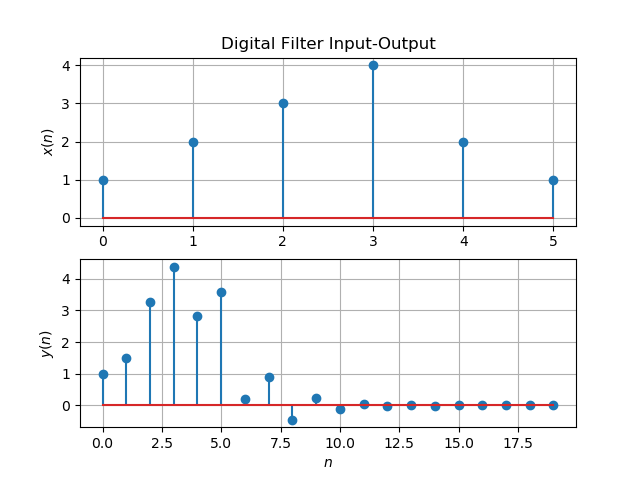
\includegraphics[width=\columnwidth]{./figs/xnyn.png}
\end{center}
\captionof{figure}{}
\label{fig:xnyn.png}	
\end{figure}

\end{enumerate}


\section{$Z$-Transform}
\begin{enumerate}[label=\thesection.\arabic*,ref=\thesection.\theenumi]

\item The $Z$-transform of $x(n)$ is defined as
\begin{equation}
\label{eq:z_trans}
X(z)={\mathcal {Z}}\{x(n)\}=\sum _{n=-\infty }^{\infty }x(n)z^{-n}
\end{equation}
Show that
\begin{equation}
\label{eq:shift1}
{\mathcal {Z}}\{x(n-1)\} = z^{-1}X(z)
\end{equation}
and find
\begin{equation}
	{\mathcal {Z}}\{x(n-k)\} 
\end{equation}
\solution From (\ref{eq:z_trans}),

\begin{align}
{\mathcal {Z}}\{x(n-1)\} & =\sum _{n=-\infty }^{\infty }x(n-1)z^{-n}\\
&= \sum _{n=-\infty }^{\infty }x(n)z^{-n-1} = z^{-1}\sum _{n=-\infty }^{\infty }x(n)z^{-n}
\end{align}

resulting in \eqref{eq:shift1}. Similarly, it can be shown that

\begin{equation}
\label{eq:z_trans_shift}
	{\mathcal {Z}}\{x(n-k)\} = z^{-k}X(z)
\end{equation}

\item Obtain $X(z)$ for $x(n)$ defined from 3.1.\\

\solution From 3.1,
\begin{align*}
x(n) = \cbrak{\underset{\uparrow}{1},2,3,4,2,1}
\end{align*}
and from \eqref{eq:z_trans}, and for given $x(n)$ we have,

\begin{align}
X(n) &= {\mathcal{Z}}\{x(n)\}\\
&= 1 + 2z^{-1} + 3z^{-2} + 4z^{-3} + 2z^{-4} + z^{-5}
\end{align}



\item Find

\begin{equation}
\label{eq:hzz}
H(z) = \frac{Y(z)}{X(z)}
\end{equation}

from  \eqref{eq:iir_filter} assuming that the $Z$-transform is a linear operation.\\
\solution  Applying \eqref{eq:z_trans_shift} in \eqref{eq:iir_filter},
\begin{align}
Y(z) + \frac{1}{2}z^{-1}Y(z) &= X(z)+z^{-2}X(z)
\\
\implies \frac{Y(z)}{X(z)} &= \frac{1 + z^{-2}}{1 + \frac{1}{2}z^{-1}}
\label{eq:freq_resp}
\end{align}
\ \\


\item Find the Z transform of 
\begin{equation}
\delta(n)
=
\begin{cases}
1 & n = 0
\\
0 & \text{otherwise}
\end{cases}
\end{equation}
and show that the $Z$-transform of
\begin{equation}
\label{eq:unit_step}
u(n)
=
\begin{cases}
1 & n \ge 0
\\
0 & \text{otherwise}
\end{cases}
\end{equation}
is
\begin{equation}
U(z) = \frac{1}{1-z^{-1}}, \quad \abs{z} > 1
\end{equation}
\solution It is easy to show that
\begin{equation}
\delta(n) \ztrans 1
\end{equation}
and from \eqref{eq:unit_step},
\begin{align}
U(z) &= \sum _{n= 0}^{\infty}z^{-n}
\\
&=\frac{1}{1-z^{-1}}, \quad \abs{z} > 1
\end{align}
using the fomula for the sum of an infinite geometric progression.\\

\item Show that 
\begin{equation}
\label{eq:anun}
a^nu(n) \ztrans \frac{1}{1-az^{-1}} \quad \abs{z} > \abs{a}
\end{equation}
\solution From \eqref{eq:unit_step}, we get,

\begin{equation}
\label{eq:anuncs}
a^nu(n)
=
\begin{cases}
a^n & n \ge 0
\\
0 & \text{otherwise}
\end{cases}
\end{equation}

from above, 
\begin{align}
U_a(z) &= \sum _{n= 0}^{\infty}a^nz^{-n}\\
&= \sum _{n= 0}^{\infty}(az^{-1})^n = \frac{1}{1-az^{-1}}, \quad \abs{z} > 1
\end{align}
using the fomula for the sum of an infinite geometric progression.\\


\item 
Let
\begin{equation}
H\brak{e^{\j \omega}} = H\brak{z = e^{\j \omega}}.
\end{equation}
Plot $\abs{H\brak{e^{\j \omega}}}$.  Comment.  $H(e^{\j \omega})$ is
known as the {\em Discret Time Fourier Transform} (DTFT) of $x(n)$.
\\
\solution The following code plots Fig. \ref{fig:dtft}.\\

\begin{lstlisting}
wget https://github.com/HARI-donk-EY/sig_pros/blob/main/codes/4/dtft.py
\end{lstlisting}
We can note that the graph in Fig. \ref{fig:dtft} is an even periodic function.\\
From the equations \label{eq:hzz} and \label{eq:freq_resp} we get,
\begin{align}
\left|H\brak{e^{\j\omega}}\right| &= \left|\frac{1 + e^{-2\j\omega}}{1 + \frac{1}{2}e^{-\j\omega}}\right| \\
&= \left|\frac{1 + \cos(-2\omega) + j\sin(-2\omega)}{1 + \frac{1}{2}(\cos(-\omega) + j\sin(-\omega))}\right|\\
&= \sqrt{\frac{\brak{1 + \cos{2\omega}}^2 + \brak{\sin{2\omega}}^2}{\brak{1 + \frac{1}{2}\cos{\omega}}^2 + \brak{\frac{1}{2}\sin{\omega}}^2}}\\
&= \sqrt{\frac{2\brak{1 + \cos{2\omega}}}{\frac{5}{4} + \cos{\omega}}} \\
&= \sqrt{\frac{2\brak{2\cos^2{\omega}}}{\frac{5}{4} + \cos{\omega}}} \\
&= \frac{4|\cos{\omega}|}{\sqrt{5 + 4\cos{\omega}}}
\end{align}
and so its fundamental period is $2\pi$.\\
\begin{figure}[!ht]
\centering
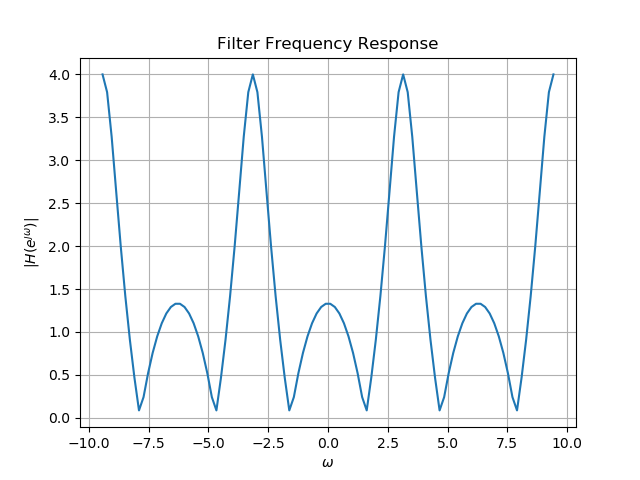
\includegraphics[width=\columnwidth]{./figs/dtft}
\caption{$\abs{H\brak{e^{\j\omega}}}$}
\label{fig:dtft}
\end{figure}


\item Express $h(n)$ in terms of $H(e^{jw})$.\\
\solution $h(n)$ is given by the inverse DTFT (IDTFT) of $H\brak{e^{\j\omega}}$
\begin{align}
h(n) &= \frac{1}{2\pi} \int_{-\pi}^{\pi} H\brak{e^{j\omega}} e^{j\omega n} \ \text{d}\omega 
\end{align}
We can prove this from \eqref{eq:z_trans},
\begin{align}
H(e^{jw}) &= \sum_{k=-\infty}^\infty h(k) e^{-j\omega k}\\
\end{align}
multiplying both sides with $e^{-j\omega k}$ and integrating w.r.t. $\omega$.\\
\begin{align}
\int_{-\pi}^{\pi} H(e^{jw}) e^{j\omega k} \text{d}\omega &= \sum_{k=-\infty}^\infty h(k) \int_{-\pi}^{\pi} e^{-j\omega n} e^{j\omega k} \text{d}\omega \\
&= \sum_{k=-\infty}^\infty h(k) \int_{-\pi}^{\pi} e^{-j\omega (n-k)}  \text{d}\omega
\end{align}
we know that $e^{-j\omega (n-k)}$ is an odd function so integration would be zero for all values of $\omega (n-k) \neq 0$, but $1$ if $\omega (n-k) = 0$.\\
\begin{align*}
\int_{-\pi}^{\pi} e^{-j\omega (n-k)}  \text{d}\omega =
\begin{cases}
0 & if n-k \neq 0\\
1 & if n-k = 0
\end{cases}
\end{align*}
From this we can complete the summation.\\

\begin{align}
\int_{-\pi}^{\pi} H(e^{jw}) e^{j\omega k} \text{d}\omega &= \sum_{k=-\infty}^\infty h(k) \int_{-\pi}^{\pi} e^{-j\omega (n-k)}  \text{d}\omega\\
&= h(n) \int_{-\pi}^{\pi} \text{d}\omega\\
& = h(n) 2\pi\\
h(n) &= \frac{1}{2\pi}\int_{-\pi}^{\pi} H(e^{jw}) e^{j\omega k} \text{d}\omega 
\end{align}
Hence proved.\\
\end{enumerate}


\section{Impulse Response}
\begin{enumerate}[label=\thesection.\arabic*]

\item Using long division, find
\begin{align}
	h(n), \quad n < 5
\end{align}
for H(z) in 
\eqref{eq:freq_resp}.

\solution
\begin{equation}
	H(z) = \frac{1 + z^{-2}}{1 + \frac12 z^{-1}}
\end{equation}
Substitute $z^{-1} = x$\\

\polylongdiv{1+x^2}{1+\frac{1}{2} x}\\

So, 

\begin{align}
H(z) & = -4 + 2z^{-1} + \frac{5}{1+ \frac{1}{2}z^{-1}}\\
& = -4 + 2z^{-1} + 5\sum_{n=0}^{\infty}\left(\frac{-1}{2}\right)^n z^{-n}\\
& = 1 - \frac{1}{2}z^{-1} + 5\sum_{n=2}^{\infty}\left(\frac{-1}{2}\right)^n z^{-n}\\
& = \sum_{n=0}^{\infty}\left(\frac{-1}{2}\right)^n z^{-n} + 4\sum_{n=2}^{\infty}\left(\frac{-1}{2}\right)^n z^{-n}\\
& = \sum_{n=-\infty}^{\infty}u(n)\left(\frac{-1}{2}\right)^n z^{-n} + \sum_{n=-\infty}^{\infty}u(n-2)\left(\frac{-1}{2}\right)^{n-2} z^{-n}
\end{align}

Therefore from \eqref{eq:z_trans},

\begin{align}
h(n) = & \left(\frac{-1}{2}\right)^nu(n) + \left(\frac{-1}{2}\right)^{n-2}u(n-2)
\end{align}
\ \\

\item \label{prob:impulse_resp}
Find an expression for $h(n)$ using $H(z)$, given that 
%in Problem \ref{eq:ztransab} and \eqref{eq:anun}, given that
\begin{equation}
\label{eq:impulse_resp}
h(n) \ztrans H(z)
\end{equation}
and there is a one to one relationship between $h(n)$ and $H(z)$. $h(n)$ is known as the {\em impulse response} of the
system defined by \eqref{eq:iir_filter}.\\Take $H(z)$ from \eqref{eq:hzz}
\\
\solution From \eqref{eq:freq_resp},
\begin{align}
H(z) &= \frac{1}{1 + \frac{1}{2}z^{-1}} + \frac{ z^{-2}}{1 + \frac{1}{2}z^{-1}}
\\
\implies h(n) &= \brak{-\frac{1}{2}}^{n}u(n) + \brak{-\frac{1}{2}}^{n-2}u(n-2)
\end{align}
using \eqref{eq:anun} and \eqref{eq:z_trans_shift}.
Let,
\begin{align}
h(n) & = h_1(n) + h_2(n)
\end{align}
Where,
\begin{align}
h_1(n) &= \left(-\frac{1}{2}\right)^nu(n)\\
h_1(n) &= \left(-\frac{1}{2}\right)^{n-2}u(n-2)
\end{align}
Then ROC of $h_1(n)$ and $h_2(n)$ will both be $|z|>|-\frac{1}{2}|$.\\
Hence ROC of $H(z)$ is $|z|>\frac{1}{2}$\\

\item Sketch $h(n)$. Is it bounded? Justify theoretically. 
\\
\solution The following code plots Fig. \ref{fig:hn}.
\begin{lstlisting}
wget https://github.com/HARI-donk-EY/sig_pros/blob/main/codes/5/hn.py
\end{lstlisting}
We know,\\
\begin{align*}
h(n) &= \brak{-\frac{1}{2}}^{n}u(n) + \brak{-\frac{1}{2}}^{n-2}u(n-2)
\end{align*}
then,
\begin{align}
\lim_{n\to\infty} h(n) &= \lim_{n\to\infty}\brak{-\frac{1}{2}}^{n}u(n) + \lim_{n\to\infty}\brak{-\frac{1}{2}}^{n-2}u(n-2)\\
h(n) &=
\begin{cases}
5\left(\frac{-1}{2}\right)^n   & n \geq 2\\ \\
\left(\frac{-1}{2}\right)^n    & 0 \leq n < 2\\ \\
0 & n < 0
\end{cases}
\end{align}
\ \\
\begin{figure}[!ht]
\centering
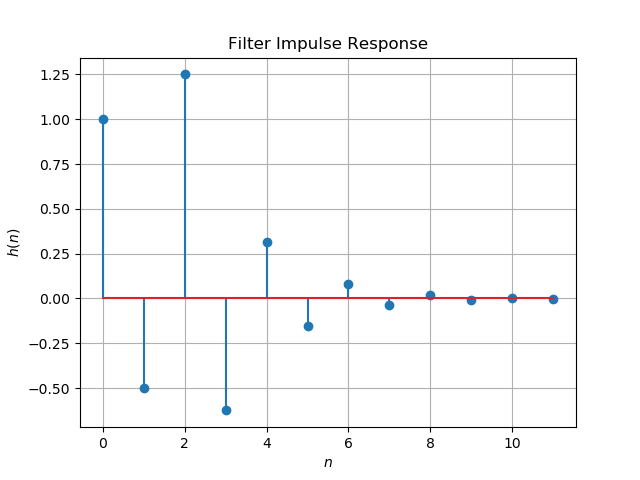
\includegraphics[width=\columnwidth]{./figs/hn}
\caption{$h(n)$ as the inverse of $H(z)$}
\label{fig:hn}
\end{figure}


\item Is $h(n)$ convergent? Justify using ratio test.\\
\solution
\begin{align}
h(n) &= \brak{-\frac{1}{2}}^{n}u(n) + \brak{-\frac{1}{2}}^{n-2}u(n-2)
\end{align}
If $L=\lim_{n\to\infty}\left|\frac{h(n+1)}{h(n)}\right| < 1$, then $h(n)$ is convergent.

\begin{align}
L &= \lim_{n\to\infty}\left|\frac{h(n+1)}{h(n)}\right|\\
&= \lim_{n\to\infty}\left|\frac{\left(-\frac{1}{2}\right)^{n+1}u(n+1)+\left(-\frac{1}{2}\right)^{n-1}u(n-1)}{\left(-\frac{1}{2}\right)^nu(n)+\left(-\frac{1}{2}\right)^{n-2}u(n-2)}\right|\\
& = \left|\frac{-\frac{1}{2}+\left(-\frac{1}{2}\right)^{-1}}{1+\left(-\frac{1}{2}\right)^{-2}}\right|\\
& = \left|\frac{-\frac{5}{2}}{5}\right|\\
& = \frac{1}{2}
\end{align}
Since $L < 1$, we can say that $h(n)$ is convergent.\\


\item The system with $h(n)$ is defined to be stable if
\begin{equation}
\sum_{n=-\infty}^{\infty}h(n) < \infty
\end{equation}
Is the system defined by \eqref{eq:iir_filter} stable for the impulse response in \eqref{eq:impulse_resp}?\\
\solution 
\begin{align}
\sum_{n=-\infty}^{\infty}h(n)&= \sum_{n=-\infty}^{\infty}\left(\brak{-\frac{1}{2}}^{n}u(n)+\brak{-\frac{1}{2}}^{n-2}u(n-2)\right)\\
&=\sum_{n=0}^{\infty}\brak{-\frac{1}{2}}^{n}u(n) + \sum_{(n-2)=0}^{\infty}\brak{-\frac{1}{2}}^{n-2}u(n-2)\\
&=2 \brak{ \frac{1}{1+\frac{1}{2}}}\\
&=\frac43
\end{align}
As $\sum_{n=-\infty}^{\infty}h(n)=\frac{4}{3}$ is less than $\infty$, the system defined by \eqref{eq:iir_filter} is stable for the impulse response in \eqref{eq:impulse_resp}.\\

\item Verify the above result using a python code.
\solution The following code determines if it is convergent or not:
\begin{lstlisting}
wget https://github.com/HARI-donk-EY/sig_pros/blob/main/codes/5/new.py
\end{lstlisting}

\item 
Compute and sketch $h(n)$ using 
\begin{equation}
\label{eq:iir_filter_h}
h(n) + \frac{1}{2}h(n-1) = \delta(n) + \delta(n-2), 
\end{equation}
%
This is the definition of $h(n)$.
\\
\solution The following code plots Fig. \ref{fig:hndef}. Note that this is the same as Fig. 
\ref{fig:hn}. 
%
\begin{lstlisting}
wget https://github.com/HARI-donk-EY/sig_pros/blob/main/codes/5/hndef.py
\end{lstlisting}
\begin{figure}[!ht]
\centering
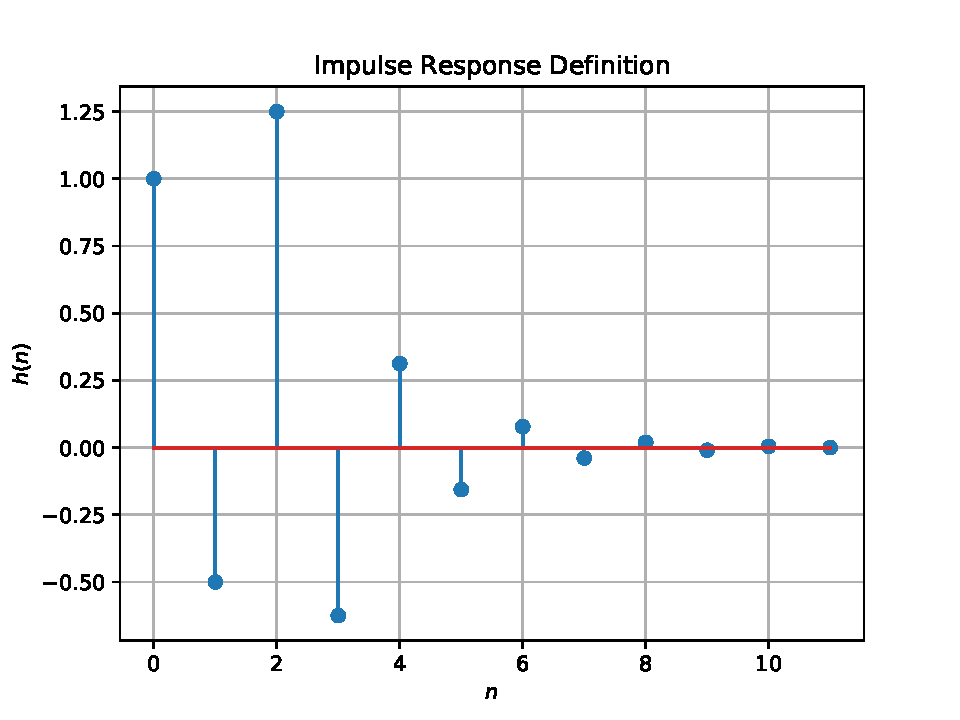
\includegraphics[width=\columnwidth]{./figs/hndef}
\caption{$h(n)$ from the definition}
\label{fig:hndef}
\end{figure}
Computing,
\begin{align*}
h(0)=1\\
h(1)=-\frac{1}{2}h(0)\\
h(2)=-\frac{1}{2}h(1)+1\\
Parallely, h(n)=-\frac{1}{2}h(n-1)\\
\end{align*}

\item Compute 
%
\begin{equation}
\label{eq:convolution}
y(n) = x(n)*h(n) = \sum_{n=-\infty}^{\infty}x(k)h(n-k)
\end{equation}
%
Comment. The operation in \eqref{eq:convolution} is known as
{\em convolution}.
%
\\
\solution The following code plots Fig. \ref{fig:ynconv.png}. Note that this is the same as 
$y(n)$ in  Fig. 
\ref{fig:xnyn.png}. 
%
\begin{lstlisting}
wget https://github.com/HARI-donk-EY/sig_pros/blob/main/codes/5/ynconv.py
\end{lstlisting}
\begin{figure}[!ht]
\centering
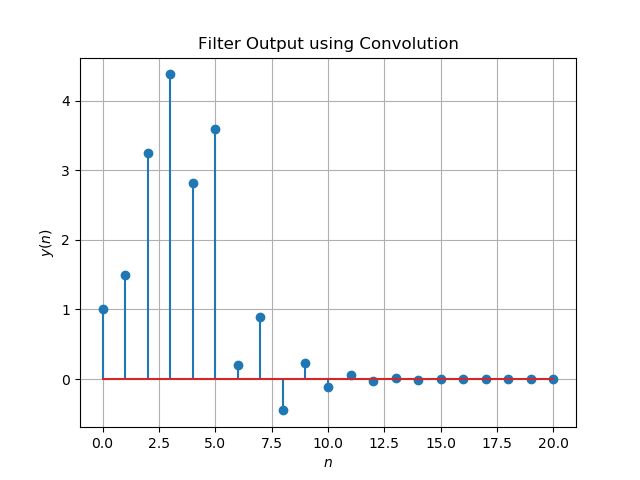
\includegraphics[width=\columnwidth]{./figs/ynconv.png}
\caption{$y(n)$ from the definition of convolution}
\label{fig:ynconv.png}
\end{figure}

\item Express the above convolution using a toeplitz matrix.
\solution
\begin{align}
\vec{y} = \vec{x} \circledast \vec{h}\\
& \vec{y} = \myvec{ h_1 & 0 & . & . & . & 0 \\ h_2 & h_1 & . & . & . & 0 \\ h_3 & h_2 & h_1 & . & . & 0 \\ h_{m-1} & . & . & . & h_2 & h_1 \\ h_m & h_{m-1} &. & . & . & h_2 \\ . & . &. & . & . & . \\ . & . & . & . & . & . \\ 0 & 0 & . & . & . & h_m } \myvec{x_1 \\ x_2 \\ . \\ . \\ . \\ . \\ x_n}
\end{align}
\begin{align}
\vec{y}&=\myvec{1 & 0&0 & 0 & 0 & 0 \\ \frac{-1}{2} & 1&0&0&0&0\\\frac{5}{4}&\frac{-1}{2}&1&0&0&0\\\frac{-5}{8}&\frac{5}{4}&\frac{-1}{2}&1&0&0\\\frac{5}{16}&\frac{-5}{8}&\frac{5}{4}&\frac{-1}{2}&1&0\\ \frac{-5}{32}&\frac{5}{16}&\frac{-5}{8}&\frac{5}{4}&\frac{-1}{2}&1\\\frac{5}{64}&\frac{-5}{32}&\frac{5}{16}&\frac{-5}{8}&\frac{5}{4}&\frac{-1}{2}\\ 0&\frac{5}{64}&\frac{-5}{32}&\frac{5}{16}&\frac{-5}{8}&\frac{5}{4}\\0&0&\frac{5}{64}&\frac{-5}{32}&\frac{5}{16}&\frac{-5}{8}\\0&0&0&\frac{5}{64}&\frac{-5}{32}&\frac{5}{16}\\0&0&0&0&\frac{5}{64}&\frac{-5}{32}\\0&0&0&0&0&\frac{5}{64}}\myvec{1\\2\\3\\4\\2\\1}
&=\myvec{1.   \\     1.5\\3.25\\4.375\\2.8125   \\3.59375\\   0.203125\\
  0.9375  \\ -0.390625 \\ 0.3125   \\ 0.     \\	   0.078125}
\end{align}
And this is what we got in \eqref{eq:convolution}

\item Show that
\begin{equation}
y(n) =  \sum_{n=-\infty}^{\infty}x(n-k)h(k)
\end{equation}

\solution 
From \eqref{eq:convolution}, we substitute $k := n - k$ to get
\begin{align}
y\brak{n} &= \sum_{k=-\infty}^{\infty}x\brak{k}h\brak{n - k} \\
		  &= \sum_{n - k=-\infty}^{\infty}x\brak{n - k}h\brak{k} \\
		  &= \sum_{k=-\infty}^{\infty}x\brak{n - k}h\brak{k}
\end{align}
\ \\
\end{enumerate}

\section{DFT}
\begin{enumerate}[label=\thesection.\arabic*]

\item
Compute
\begin{equation}
X(k) \define \sum _{n=0}^{N-1}x(n) e^{-\j2\pi kn/N}, \quad k = 0,1,\dots, N-1
\end{equation}
and $H(k)$ using $h(n)$.

\solution 
The following code generates the data required for plotting.
\begin{lstlisting}
wget https://github.com/HARI-donk-EY/sig_pros/blob/main/codes/6/header.h
wget https://github.com/HARI-donk-EY/sig_pros/blob/main/codes/6/6.1/XkHk_dat.c 
\end{lstlisting}

The following code plots Fig. \ref{fig:xkhk}. 
\begin{figure}[!ht]
\centering
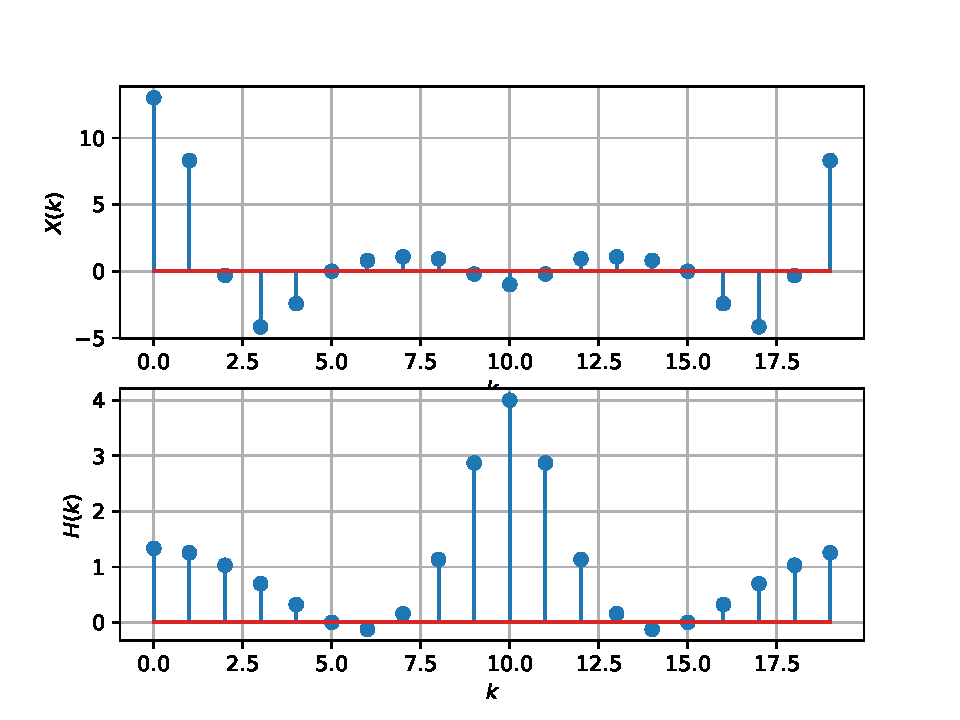
\includegraphics[width=\columnwidth]{./figs/xkhk}
\caption{$X(k) ,H(k)$ from the DFT}
\label{fig:xkhk}
\end{figure}
\begin{lstlisting}
wget https://github.com/HARI-donk-EY/sig_pros/blob/main/codes/6/6.1/XkHk.py
\end{lstlisting}
\ \\
\item
Compute 
\begin{equation}
Y(k) = X(k)H(k)
\end{equation}
\solution The following code plots Fig. \ref{fig:yk}. 
\begin{figure}[!ht]
\centering
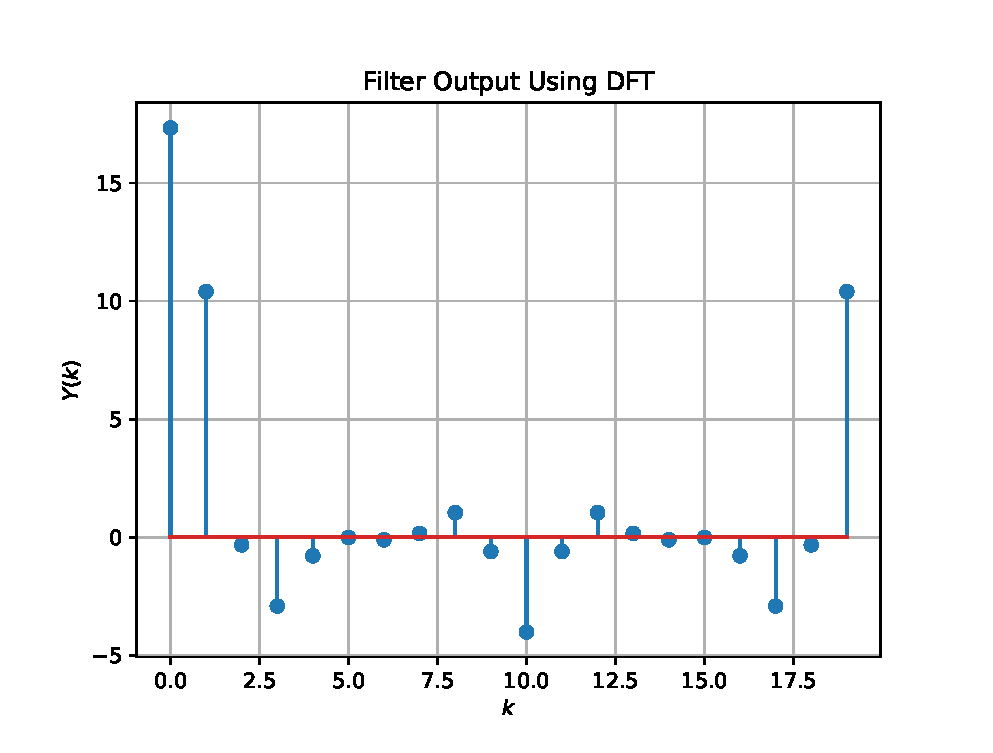
\includegraphics[width=\columnwidth]{./figs/yk}
\caption{$Y(k)$ from the DFT}
\label{fig:yk}
\end{figure}
The data can be obtained from
\begin{lstlisting}
wget https://github.com/HARI-donk-EY/sig_pros/blob/main/codes/6/header.h
wget https://github.com/HARI-donk-EY/sig_pros/blob/main/codes/6/6.2/y(k)dat.c  
\end{lstlisting}
The plotting is done by
\begin{lstlisting}
wget https://github.com/HARI-donk-EY/sig_pros/blob/main/codes/6/6.2/yk.py
\end{lstlisting}
\ \\
\item Compute
\begin{equation}
 y\brak{n}={\frac {1}{N}}\sum _{k=0}^{N-1}Y\brak{k}\cdot e^{\j 2\pi kn/N},\quad n = 0,1,\dots, N-1
\end{equation}
\solution The following code plots Fig. \ref{fig:ynconv}. Note that this is the same as 
$y(n)$ in  Fig.


\end{enumerate}

\end{document}
